\section{Motivation}

The previous chapters introduced the constrained finite time optimal control problem and showed
how it gives rise to the receding-horizon control law used in MPC. At each sampling instant,
one solves a finite-horizon optimization problem, applies only the first input of the optimal
sequence, measures the new state, and repeats the procedure. This mechanism introduces
feedback, because the optimization is repeatedly updated using the current state.\\
However, the fact that an optimization problem is solved at every time instant does not by
itself guarantee that the resulting closed-loop system behaves well. In particular, two fundamental
questions remain open. First, if the MPC problem is feasible at the current state, will it also be
feasible at the next state after applying the first optimal input? Second, will the closed-loop
trajectory actually converge to the desired equilibrium? These are the questions of recursive
feasibility and closed-loop stability.\\

The ideal objective of constrained control can be described as follows. Given a discrete-time
system
\[
    x(k+1) = g(x(k),u(k)),
\]
with state and input constraints
\[
    x(k) \in \cX, \qquad u(k) \in \cU,
\]
we would like to design a control law
\[
    u(k) = \kappa(x(k))
\]
such that the closed-loop trajectory satisfies the constraints for all times, converges to the
origin, achieves good performance, and does so from as large a set of initial conditions as
possible. In other words, the controller should not only compute locally optimal actions, but
also preserve the long-term admissibility and stability of the closed loop.\\

A natural benchmark is the constrained infinite-horizon optimal control problem
\[
\begin{aligned}
    J_\infty^\star(x(0))
    :=
    \min_{u(\cdot)} \quad
    & \sum_{i=0}^{\infty} \stagecost(x_i,u_i) \\
    \text{subj. to} \quad
    & x_{i+1} = A x_i + B u_i, \qquad i = 0,1,\ldots,\\
    & x_i \in \cX, \qquad u_i \in \cU, \qquad i = 0,1,\ldots,\\
    & x_0 = x(0).
\end{aligned}
\]
This formulation is conceptually attractive because it optimizes over the entire future. The
stage cost \(\stagecost(x,u)\) measures the immediate cost of being in state \(x\) and applying
input \(u\), while the infinite sum forces the optimizer to account for the long-term consequences
of each decision. In this sense, the infinite-horizon problem naturally balances short-term and
long-term benefits.\\
The difficulty is that the infinite-horizon problem contains infinitely many decision variables
and constraints. Except in special cases, it cannot be solved directly online. MPC therefore
replaces it by a finite-horizon problem of the form
\[
\begin{aligned}
    J^\star(x(k))
    :=
    \min_{U} \quad
    & \terminalcost(x_N) + \sum_{i=0}^{N-1} \stagecost(x_i,u_i) \\
    \text{subj. to} \quad
    & x_{i+1} = A x_i + B u_i, \qquad i = 0,\ldots,N-1,\\
    & x_i \in \cX, \qquad u_i \in \cU, \qquad i = 0,\ldots,N-1,\\
    & x_N \in \cX_f,\\
    & x_0 = x(k),
\end{aligned}
\]
where
\[
    U := \{u_0,\ldots,u_{N-1}\}.
\]
The finite horizon makes the optimization problem computable. The terminal cost
\(\terminalcost(x_N)\) and terminal set \(\cX_f\) are introduced to approximate the part of the
infinite-horizon problem that has been truncated. The main message of this chapter is that
these terminal ingredients are not merely optional tuning parameters: they are the standard
mechanism through which one recovers feasibility and stability guarantees for finite-horizon MPC.

\section{MPC: Key Points Illustrated}

Before proving recursive feasibility and stability formally, it is useful to look at what can
happen in a constrained control problem when different controllers and different MPC
formulations are used. We illustrate
these issues through the example of a Cessna
Citation aircraft. The model is a linearized continuous-time model around an operating point at
altitude \(5000\,\mathrm{m}\) and speed \(128.2\,\mathrm{m/s}\). The input is the elevator angle,
while the state variables are
\[
    x_1=\text{angle of attack}, \qquad
    x_2=\text{pitch angle}, \qquad
    x_3=\text{pitch rate}, \qquad
    x_4=\text{altitude}.
\]
The measured outputs are pitch angle and altitude. The linearized model is
\[
\dot{x}
=
\begin{bmatrix}
-1.2822 & 0 & 0.98 & 0\\
0 & 0 & 1 & 0\\
-5.4293 & 0 & -1.8366 & 0\\
-128.2 & 128.2 & 0 & 0
\end{bmatrix}x
+
\begin{bmatrix}
-0.3\\
0\\
-17\\
0
\end{bmatrix}u,
\qquad
y
=
\begin{bmatrix}
0 & 1 & 0 & 0\\
0 & 0 & 0 & 1
\end{bmatrix}x.
\]
The open-loop response is unstable, with open-loop poles
\[
    0, \quad 0, \quad -1.5594 \pm 2.29i.
\]
Therefore, some form of feedback stabilization is necessary. At the same time, the aircraft is
subject to physical and operational constraints: the elevator angle is bounded, the elevator rate
is bounded, and the pitch angle must remain within an admissible range. These constraints are
not secondary details; they determine whether the closed-loop behavior is acceptable.
\begin{figure}[htbp]
    \centering
    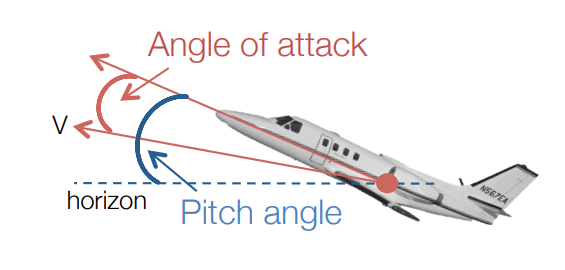
\includegraphics[width=0.6\textwidth]{images/ch07_cessna_model.png}
    \caption{Linearized Cessna Citation aircraft model used to illustrate the effect of constraints
    in MPC. The input is the elevator angle, the states are angle of attack, pitch angle, pitch rate,
    and altitude, and the outputs are pitch angle and altitude.}
    \label{fig:ch07_cessna_model}
\end{figure}
A first comparison is between unconstrained LQR and constrained linear MPC with quadratic
cost. In the LQR case, one solves the infinite-horizon quadratic problem
\[
    J_\infty^\star(x(k))
    =
    \min
    \sum_{i=0}^{\infty}
    \left(
        x_i^\top Qx_i + u_i^\top Ru_i
    \right)
\]
subject only to the dynamics
\[
    x_{i+1}=Ax_i+Bu_i,
    \qquad
    x_0=x(k).
\]
By contrast, in the finite-horizon MPC formulation one solves
\[
    J^\star(x(k))
    =
    \min_U
    \sum_{i=0}^{N-1}
    \left(
        x_i^\top Qx_i + u_i^\top Ru_i
    \right)
\]
subject to the same prediction dynamics, but also to the constraints
\[
    x_i\in\cX, \qquad u_i\in\cU,
    \qquad i=0,\ldots,N-1,
\]
with
\[
    x_0=x(k).
\]
In both cases the cost is quadratic, the dynamics are linear, and the weights satisfy
\[
    Q=Q^\top\succeq 0,
    \qquad
    R=R^\top\succ 0.
\]
The crucial difference is that LQR does not take the constraints into account during the design,
whereas MPC includes them directly in the optimization problem.\\

This distinction is important because a controller designed without constraints may behave very
poorly once constraints are imposed afterwards. For example, one might design an unconstrained
LQR controller and then simply saturate the elevator input whenever the actuator limit is
exceeded. This may seem reasonable, but it changes the closed-loop system in a way that was
not accounted for in the LQR design. In the aircraft example, starting from an altitude deviation
of \(10\,\mathrm{m}\),
\[
    x_0 =
    \begin{bmatrix}
        0 & 0 & 0 & 10
    \end{bmatrix}^\top,
\]
with sampling time \(0.25\,\mathrm{s}\), \(Q=I\), and \(R=10\), the LQR law with saturated inputs
leads to an unstable closed-loop response. Figure~\ref{fig:ch07_lqr_saturation} shows that the
altitude and pitch angle do not converge, while the elevator angle repeatedly hits the imposed
saturation bounds.\\

\begin{figure}[htbp]
    \centering
    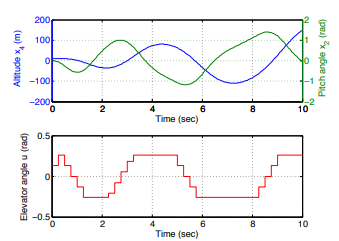
\includegraphics[width=0.6\textwidth]{images/ch07_lqr_saturation.png}
    \caption{LQR with saturated elevator angle. Although the unconstrained LQR law is
    stabilizing for the nominal unconstrained model, saturating the input afterwards can make
    the closed-loop system unstable.}
    \label{fig:ch07_lqr_saturation}
\end{figure}

MPC improves on this situation by including actuator bounds directly in the prediction problem.
For instance, suppose that the MPC controller enforces the elevator angle constraint
\[
    |u_k|\leq 0.262,
\]
corresponding approximately to \(\pm 15^\circ\), with the same weights \(Q=I\), \(R=10\), and
horizon \(N=10\). The controller now knows during the optimization that the elevator cannot
exceed its admissible range. However, this is still not enough if the actuator rate constraint is
ignored. The prediction model assumes that the input can jump freely within the admissible
interval, whereas the real actuator cannot. As shown in
Figure~\ref{fig:ch07_mpc_input_bound_only}, the resulting closed-loop trajectory does not
converge to the desired steady state, but instead approaches a limit cycle.

\begin{figure}[htbp]
    \centering
    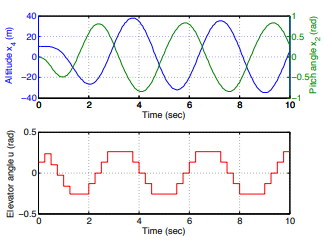
\includegraphics[width=0.6\textwidth]{images/ch07_mpc_input_bound_only.png}
    \caption{MPC with only the elevator angle bound \(|u_k|\leq 0.262\). The controller accounts
    for saturation, but not for the elevator rate constraint. As a consequence, the closed-loop
    trajectory may fail to converge and can enter a limit cycle.}
    \label{fig:ch07_mpc_input_bound_only}
\end{figure}

The next step is to include all relevant actuator constraints. In addition to the magnitude bound
on the elevator angle, one imposes a rate constraint. In discrete time, an elevator rate bound can
be approximated by
\[
    |u_i-u_{i-1}|
    \leq
    0.524\,T_s,
\]
where \(T_s\) is the sampling time. With the same horizon \(N=10\), the MPC controller now
optimizes over trajectories that are consistent with both the elevator magnitude and the elevator
rate limits. The behavior in Figure~\ref{fig:ch07_mpc_all_input_constraints} is then stable: the
altitude and pitch angle converge, and the input uses the available control authority efficiently
without violating the actuator restrictions.

\begin{figure}[htbp]
    \centering
    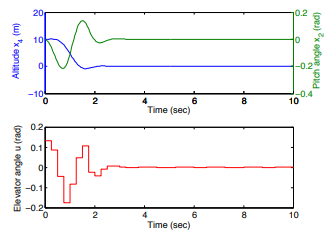
\includegraphics[width=0.6\textwidth]{images/ch07_mpc_all_input_constraints.png}
    \caption{MPC with both elevator magnitude and elevator rate constraints. Once all relevant
    actuator constraints are included in the prediction problem, the closed-loop response becomes
    stable in this example.}
    \label{fig:ch07_mpc_all_input_constraints}
\end{figure}

State constraints can be equally important. Consider a larger altitude deviation, for instance
\[
    x_0 =
    \begin{bmatrix}
        0 & 0 & 0 & 100
    \end{bmatrix}^\top.
\]
If the MPC controller includes the input magnitude and rate constraints but does not explicitly
constrain the pitch angle, it may choose a trajectory that regulates altitude by using a very large
pitch transient. In the example shown in Figure~\ref{fig:ch07_mpc_without_pitch_constraint},
the pitch angle reaches approximately \(-0.9\,\mathrm{rad}\), corresponding to about \(-50^\circ\).
Such a maneuver may be optimal for the mathematical problem that was solved, but it is not
acceptable from the physical or comfort point of view.

\begin{figure}[htbp]
    \centering
    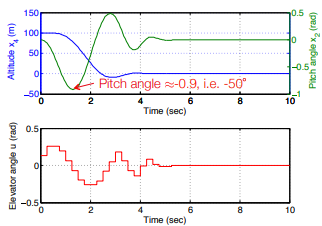
\includegraphics[width=0.6\textwidth]{images/ch07_mpc_without_pitch_constraint.png}
    \caption{MPC with input constraints but without a pitch-angle state constraint. The
    controller regulates altitude, but it produces an excessive pitch transient.}
    \label{fig:ch07_mpc_without_pitch_constraint}
\end{figure}

If one adds the passenger-comfort constraint
\[
    |x_2|\leq 0.349,
\]
then the controller must choose a different trajectory. The pitch angle constraint becomes active,
as shown in Figure~\ref{fig:ch07_mpc_with_pitch_constraint}. The altitude response is less
aggressive, but the closed-loop trajectory respects the admissible pitch range. This example
highlights one of the main advantages of MPC: constraints can be encoded directly in the
controller design, and the optimizer automatically trades performance against constraint
satisfaction.

\begin{figure}[htbp]
    \centering
    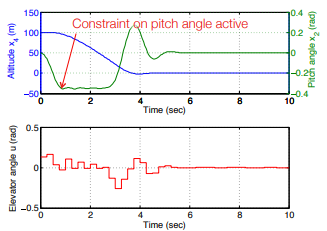
\includegraphics[width=0.6\textwidth]{images/ch07_mpc_with_pitch_constraint.png}
    \caption{MPC with input constraints and the pitch-angle constraint \(|x_2|\leq 0.349\).
    The pitch constraint becomes active during the transient, and the controller modifies the
    altitude response in order to remain feasible.}
    \label{fig:ch07_mpc_with_pitch_constraint}
\end{figure}

The final point illustrated by the aircraft example is more subtle. Even if the correct physical
constraints are included, the prediction horizon may still be too short. With the same input
constraints and rate constraints, but with horizon reduced to
\[
    N=4,
\]
the closed-loop response may again lose stability. Figure~\ref{fig:ch07_short_horizon} shows
that decreasing the prediction horizon can destroy the stabilizing behavior observed for the
longer horizon. The controller only optimizes over a short future window, and therefore it may
choose inputs that look beneficial over that window but do not lead to a good long-term
closed-loop evolution.\\

\begin{figure}[htbp]
    \centering
    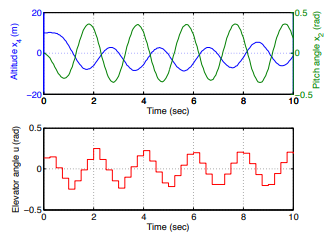
\includegraphics[width=0.6\textwidth]{images/ch07_short_horizon.png}
    \caption{MPC with all considered input constraints but short horizon \(N=4\). Reducing the
    prediction horizon can cause loss of stability, even though the constraints are included in the
    optimization problem.}
    \label{fig:ch07_short_horizon}
\end{figure}

The examples therefore show both the strength and the limitation of finite-horizon MPC. The
strength is that constraints can be incorporated directly into the control problem, instead of
being handled afterwards by saturation or ad hoc logic. This allows the controller to anticipate
constraint activation and to use the available control authority systematically. The limitation is
that constraint satisfaction over a finite prediction window does not automatically imply
constraint satisfaction and stability for all future times. A finite-horizon controller remains
short-sighted unless its terminal behavior is designed carefully.

\section{Loss of Feasibility and Stability in Finite-Horizon MPC}

The examples of the previous section suggest that MPC is a powerful framework for constrained
control, but they also reveal an important limitation. A standard finite-horizon MPC formulation
does not automatically guarantee that the optimization problem will remain feasible at all future
time instants, nor does it automatically guarantee that the closed-loop trajectory will converge
to the origin.\\

In other words, two things can go wrong. First, the MPC problem may become infeasible after
some time, even if it was feasible at the initial condition. Second, the optimization problem may
remain feasible, but the resulting closed-loop trajectory may fail to converge. These two issues
are called loss of feasibility and loss of stability, respectively.\\

The reason is that finite-horizon MPC is intrinsically a short-sighted strategy. At time \(k\), the
controller optimizes an open-loop trajectory over only \(N\) future steps. Then, however, only the
first input is applied, and the problem is solved again at the next time instant. Thus the actual
closed-loop trajectory is not the same object as the open-loop prediction computed at one time
instant. A predicted trajectory may be feasible over the finite horizon, but the first input of that
trajectory may still drive the system to a state from which the next finite-horizon problem has
no solution.

\subsection{Loss of feasibility: double integrator example}

To see how loss of feasibility can occur, consider the constrained double integrator
\[
    x(k+1)
    =
    \begin{bmatrix}
        1 & 1\\
        0 & 1
    \end{bmatrix}x(k)
    +
    \begin{bmatrix}
        0\\
        1
    \end{bmatrix}u(k),
    \qquad
    y(k)
    =
    \begin{bmatrix}
        1 & 0
    \end{bmatrix}x(k).
\]
The input is constrained by
\[
    -0.5 \leq u(k) \leq 0.5,
\]
and the state is constrained by the box
\[
    \begin{bmatrix}
        -5\\
        -5
    \end{bmatrix}
    \leq
    x(k)
    \leq
    \begin{bmatrix}
        5\\
        5
    \end{bmatrix}.
\]
We compute a receding-horizon controller with quadratic objective, horizon
\[
    N=3,
\]
terminal weight and state weight
\[
    P=Q=
    \begin{bmatrix}
        1 & 0\\
        0 & 1
    \end{bmatrix},
\]
and input weight
\[
    R=10.
\]
For each measured state \(x(k)\), the controller solves the corresponding constrained finite-time
optimal control problem, obtains an optimal input sequence
\[
    U^\star(x(k))
    =
    \{u_0^\star(x(k)),u_1^\star(x(k)),u_2^\star(x(k))\},
\]
applies only the first input \(u_0^\star(x(k))\), and repeats the procedure at the next sampling
instant.\\
The finite-horizon problem can be written as a quadratic program of the form
\[
    J^\star(x(k))
    =
    \min_U
    U^\top H U + 2x(k)^\top F U + x(k)^\top Yx(k)
\]
subject to
\[
    GU \leq w + Ex(k).
\]
The matrices \(H\), \(F\), \(Y\), \(G\), \(E\), and \(w\) are obtained by substituting the double
integrator dynamics into the cost and into the constraints. The exact entries are not conceptually
important here. What matters is that, for each value of the parameter \(x(k)\), the QP is either
feasible or infeasible. Therefore, the feasible set of the finite-horizon MPC problem is a subset
of the state constraint set.\\

Now consider the receding-horizon implementation. The algorithm is simple: measure the state,
solve the CFTOC problem, check whether a feasible optimizer exists, apply the first optimal
input, and repeat. Starting from
\[
    x(0)=
    \begin{bmatrix}
        -4\\
        3
    \end{bmatrix},
\]
the finite-horizon problem is feasible and gives
\[
    u_0^\star(x(0))=-0.5.
\]
After applying this input, the system evolves to
\[
    x(1)=
    \begin{bmatrix}
        -1\\
        2.5
    \end{bmatrix},
\]
and the MPC problem is again feasible, with
\[
    u_0^\star(x(1))=-0.5.
\]
After applying this second input, the system reaches
\[
    x(2)=
    \begin{bmatrix}
        1.5\\
        2
    \end{bmatrix}.
\]
At this point, however, the finite-horizon problem is infeasible. Thus the controller has driven
the system from a feasible initial state to a state at which the next optimization problem has no
solution.\\
\begin{figure}[htbp]
    \centering
    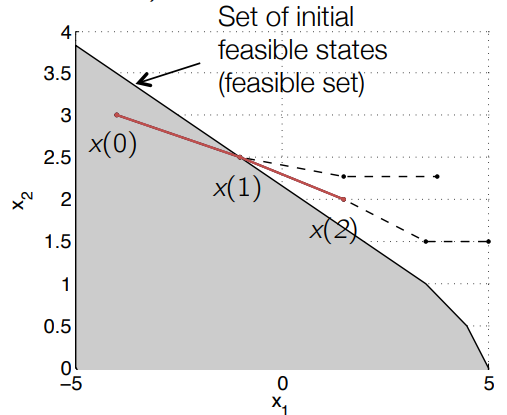
\includegraphics[width=0.5\textwidth]{images/ch07_double_integrator_infeasible_trajectory.png}
    \caption{Closed-loop evolution of the double integrator under finite-horizon MPC. Although
    \(x(0)\) and \(x(1)\) are feasible, the state \(x(2)\) lies outside the finite-horizon feasible set,
    so the next MPC problem is infeasible.}
    \label{fig:ch07_double_integrator_infeasible_trajectory}
\end{figure}
This example is important because no disturbance or model mismatch is involved. The system
evolves exactly according to the model used inside the optimizer. The loss of feasibility is
therefore not caused by uncertainty, but by the finite prediction horizon itself. The controller
can see only three steps ahead, and the first input of a three-step feasible plan does not
necessarily lead to a state from which another three-step feasible plan exists.\\

The same phenomenon can be visualized by sampling many initial states. Some initial states
lead to closed-loop trajectories for which the MPC problem remains feasible at every time
instant; others lead to trajectories that eventually become infeasible. In
Figure~\ref{fig:ch07_double_integrator_grid}, the boxes represent initial conditions that lead to
feasible closed-loop trajectories, while the circles represent initial conditions that do not. The
figure shows that the set of states from which the finite-horizon problem is feasible is not
automatically the same as the set of states from which the receding-horizon closed loop remains
feasible forever.

\begin{figure}[htbp]
    \centering
    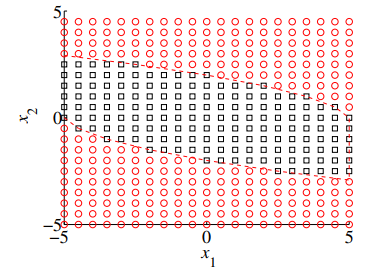
\includegraphics[width=0.5\textwidth]{images/ch07_double_integrator_grid.png}
    \caption{Sampled initial conditions for the double integrator. Boxes denote states leading to
    feasible closed-loop trajectories, while circles denote states for which the MPC problem becomes
    infeasible after some time.}
    \label{fig:ch07_double_integrator_grid}
\end{figure}

\begin{theorembox}[Recursive feasibility]
A finite-horizon MPC controller is recursively feasible on a set \(\Omega\) if feasibility propagates
forward in closed loop. More precisely, whenever the MPC problem is feasible at
\(x(k)\in\Omega\), the successor state
\[
    x(k+1)=Ax(k)+Bu_0^\star(x(k))
\]
must also belong to the feasible set of the MPC problem. The double integrator example shows
that standard finite-horizon MPC does not automatically have this property.
\end{theorembox}

\subsection{Feasibility and stability depend on the tuning}

Loss of feasibility is not the only possible failure. Even when the finite-horizon optimization
problem remains feasible, the resulting trajectories may not converge to the origin. The stability
properties of finite-horizon MPC can depend strongly on the horizon length and on the cost
weights.\\
Consider the unstable system
\[
    x(k+1)
    =
    \begin{bmatrix}
        2 & 1\\
        0 & 0.5
    \end{bmatrix}x(k)
    +
    \begin{bmatrix}
        1\\
        0
    \end{bmatrix}u(k),
\]
with input constraint
\[
    -1 \leq u(k) \leq 1,
\]
state constraint
\[
    \begin{bmatrix}
        -10\\
        -10
    \end{bmatrix}
    \leq
    x(k)
    \leq
    \begin{bmatrix}
        10\\
        10
    \end{bmatrix},
\]
and state weight
\[
    Q=
    \begin{bmatrix}
        1 & 0\\
        0 & 1
    \end{bmatrix}.
\]
The purpose of this example is to investigate the stability properties of the finite-horizon
receding-horizon controller for different horizons \(N\) and different input weights \(R\).

% Create three subfigures on the same row, with the same width and height, and with a common legend on the right
\begin{figure}[htbp]
    \centering 
    \begin{subfigure}[t]{0.31\textwidth}
        \centering
        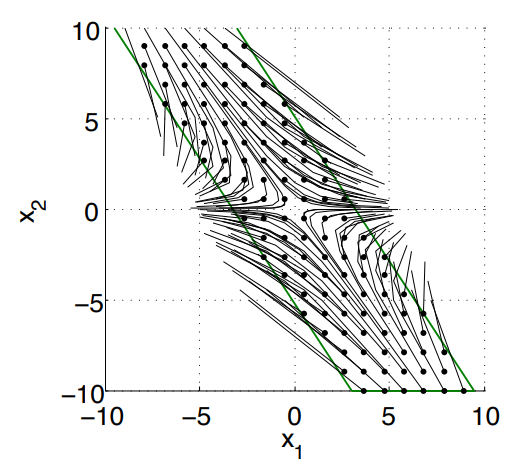
\includegraphics[width=\linewidth]{images/ch07_tuning_R10_N2.png}
        \caption{\(R=10\), \(N=2\)}
    \end{subfigure}
    \hfill
    \begin{subfigure}[t]{0.31\textwidth}
        \centering
        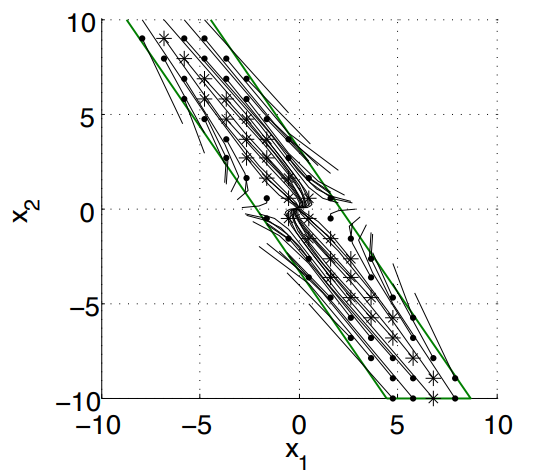
\includegraphics[width=\linewidth]{images/ch07_tuning_R2_N3.png}
        \caption{\(R=2\), \(N=3\)}
    \end{subfigure}
    \hfill
    \begin{subfigure}[t]{0.31\textwidth}
        \centering
        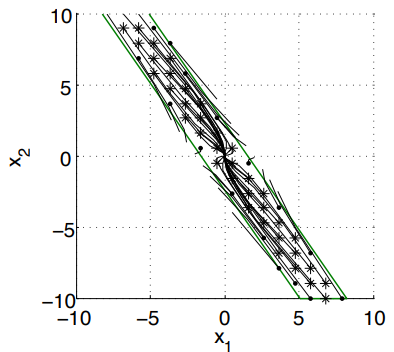
\includegraphics[width=\linewidth]{images/ch07_tuning_R1_N4.png}
        \caption{\(R=1\), \(N=4\)}
    \end{subfigure}
        \caption{Effect of horizon length and input weight on finite-horizon MPC. Stars denote
    initial points with convergent trajectories, while circles denote initial points that diverge.
    The green lines denote the feasible set of initial states.}
    \label{fig:ch07_tuning_results_subfigures}
\end{figure}

The results are summarized in Figure~\ref{fig:ch07_tuning_results_subfigures}. For
$
    R=10, N=2,
$
all sampled trajectories are unstable. In this case the horizon is very short and the input penalty
is large, so the controller is too short-sighted and too conservative to stabilize the unstable
mode. For
$
    R=2,N=3,
$
some trajectories converge, while others still diverge. Finally, for
$
    R=1, N=4,
$
a larger portion of the sampled initial conditions leads to convergent trajectories.\\

The green boundary in the plots denotes the set of feasible initial points. This feasible set
depends on the horizon \(N\), because a longer horizon changes the set of states from which it
is possible to find an admissible predicted trajectory. However, the feasible set does not depend
on the input weight \(R\), since feasibility is determined by the dynamics and constraints, not
by the objective function. The actual closed-loop stability behavior, on the other hand, depends
on both \(N\) and \(R\). Thus the cost affects which feasible trajectory is selected, and therefore
it affects the closed-loop trajectory.

\begin{figure}[htbp]
    \centering
    \begin{subfigure}[t]{0.45\textwidth}
        \centering
        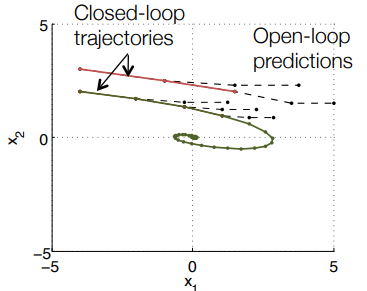
\includegraphics[width=\linewidth]{images/ch07_open_loop_closed_loop_trajectories.png}
        \caption{Open-loop predictions and resulting closed-loop trajectories.}
        \label{fig:ch07_open_loop_closed_loop_trajectories}
    \end{subfigure}
    \hfill
    \begin{subfigure}[t]{0.45\textwidth}
        \centering
        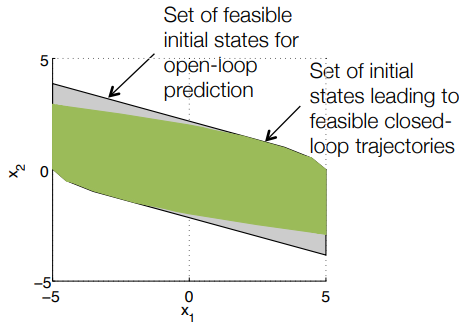
\includegraphics[width=\linewidth]{images/ch07_open_loop_closed_loop_feasible_sets.png}
        \caption{Open-loop feasible states and states leading to feasible closed-loop trajectories.}
        \label{fig:ch07_open_loop_closed_loop_feasible_sets}
    \end{subfigure}
    \caption{Mismatch between finite-horizon open-loop prediction and receding-horizon closed-loop behavior. 
    The left plot shows that the predicted open-loop trajectories need not coincide with the closed-loop
    trajectories generated by repeatedly resolving the MPC problem. The right plot shows that the set of
    initial states admitting a feasible finite-horizon open-loop prediction can differ from the set of initial
    states that lead to feasible closed-loop trajectories.}
    \label{fig:ch07_open_loop_vs_closed_loop}
\end{figure}
This example highlights an important point. Feasibility and stability are related, but they are
not equivalent. A state may be feasible for the finite-horizon optimization problem, but the
resulting closed-loop trajectory may still fail to converge. Conversely, changing the cost weights
can change the closed-loop behavior even though it does not change the feasible set. The tuning
parameters of finite-horizon MPC therefore have a complex effect on the resulting trajectories.

\subsection{Why finite-horizon MPC is short-sighted}

The previous examples can be summarized geometrically. At time \(k\), the controller computes
an open-loop prediction over a finite horizon. This prediction may satisfy all constraints over
the predicted window. However, after the first input is applied and the problem is solved again,
the closed-loop trajectory may deviate from what would have been expected by considering only
one finite open-loop plan.\\

This is the central mismatch: the set of initial states from which there exists a feasible
open-loop prediction over \(N\) steps is generally larger than, or at least different from, the set of
initial states from which the receding-horizon closed loop remains feasible for all times. The
finite-horizon problem certifies only that a feasible path exists over the next \(N\) steps. It does
not automatically certify that feasibility can be maintained after those \(N\) steps.\\

The ideal solution would be to solve the constrained infinite-horizon problem. If the horizon
were infinite, the open-loop plan would already contain the entire future. After applying the
first input, the remaining tail of the infinite-horizon plan would still be a feasible candidate at
the next time step. Therefore, if the infinite-horizon problem is feasible initially, the closed-loop
trajectory remains feasible. Moreover, if the infinite-horizon cost is finite and the stage cost is
positive definite, then the state and input must converge asymptotically to the origin.\\

For a finite horizon, this argument no longer holds automatically. The controller approximates
the infinite-horizon strategy, but because it sees only a finite window, it may make decisions
that are locally reasonable and globally poor. This is why standard finite-horizon receding
horizon control may lose feasibility or stability.

\begin{theorembox}[Finite versus infinite horizon]
With an infinite horizon, the tail of the optimal trajectory provides a natural feasible candidate
after the first input has been applied. This gives feasibility and stability properties. With a
finite horizon, this tail is missing. The controller is short-sighted, and recursive feasibility and
stability must be enforced by design.
\end{theorembox}

\subsection{The role of terminal cost and terminal constraints}

The standard solution is to modify the finite-horizon problem so that it mimics the infinite-horizon
problem beyond the end of the prediction window. This is done by adding a terminal cost and a
terminal constraint:
\[
\begin{aligned}
    J^\star(x(k))
    =
    \min_U \quad
    & \terminalcost(x_N)
    +
    \sum_{i=0}^{N-1}\stagecost(x_i,u_i) \\
    \text{subj. to} \quad
    & x_{i+1}=Ax_i+Bu_i,
    \qquad i=0,\ldots,N-1,\\
    & x_i\in\cX,
    \qquad
    u_i\in\cU,
    \qquad i=0,\ldots,N-1,\\
    & x_N\in\cX_f,\\
    & x_0=x(k).
\end{aligned}
\]
The terminal cost \(\terminalcost(x_N)\) approximates the cost of controlling the system after
the end of the finite horizon. The terminal set \(\cX_f\) approximates the set of terminal states
from which the constraints can be satisfied indefinitely by a suitable local controller. In this
sense, the terminal ingredients are a way of ``faking'' the infinite horizon while keeping the
optimization problem finite-dimensional and computationally tractable.\\
The rest of the chapter makes this idea precise. We will show that, if the terminal set is chosen
to be invariant under a suitable local control law and if the terminal cost decreases along that
local closed loop, then the finite-horizon MPC controller is recursively feasible and stabilizing.
The proof relies on a simple but powerful idea: shift the previously optimal input sequence by
one step and append the terminal control law at the end. This shifted sequence provides
recursive feasibility, while the decrease of the optimal cost provides a Lyapunov function.

\section{Feasibility and Stability Guarantees in MPC}

After seeing that finite-horizon MPC may lose feasibility or stability, we now turn to the
standard mechanism used to recover guarantees. The key tool is Lyapunov stability theory.
The reason is that, in MPC, the optimal value function naturally behaves like an energy
function: if it can be shown to decrease along the closed-loop trajectory, then it can be used
to prove asymptotic stability.

\subsection{Lyapunov Stability Revisited}

Consider a nonlinear, time-invariant, discrete-time autonomous system
\[
    x(k+1)=g(x(k)).
\]
Let \(\bar{x}\) be an equilibrium point, meaning that
\[
    g(\bar{x})=\bar{x}.
\]
We are interested in understanding whether trajectories starting near \(\bar{x}\), or more
generally inside a given set \(\Omega\), remain well behaved and converge to \(\bar{x}\).

\begin{theorembox}[Asymptotic stability]
An equilibrium point \(\bar{x}\in\Omega\) of the system
\[
    x(k+1)=g(x(k))
\]
is called \emph{asymptotically stable in the positive invariant set}
\(\Omega\subseteq\R^n\) if it is Lyapunov stable and attractive in \(\Omega\), that is,
\[
    \lim_{k\to\infty}\norm{x(k)-\bar{x}}=0,
    \qquad
    \forall x(0)\in\Omega.
\]
If the same property holds with \(\Omega=\R^n\), then the equilibrium is called
\emph{globally asymptotically stable}.
\end{theorembox}

The set \(\Omega\) is important because, in constrained MPC, stability is usually not global in
\(\R^n\). The state cannot be arbitrary: it must remain inside the constraint set and inside the
set of states for which the MPC problem is feasible. Therefore, the natural stability statement
for constrained MPC is stability on a positively invariant feasible set, rather than global
stability on the whole state space.

A standard way to prove asymptotic stability is to construct a Lyapunov function. The
interpretation is the same as in the earlier system-theory chapter: the Lyapunov function is a
generalized energy. It is positive away from the equilibrium and decreases along trajectories.
For simplicity, and in line with the MPC regulation problem, we state the definition for the
equilibrium at the origin.

\begin{theorembox}[Lyapunov function]
Consider the equilibrium point \(\bar{x}=0\) of
\[
    x(k+1)=g(x(k)).
\]
Let \(\Omega\subset\R^n\) be a closed and bounded positive invariant set containing the origin.
A function
\[
    V:\R^n\to\R
\]
is called a Lyapunov function in \(\Omega\) if it is continuous at the origin, finite for every
\(x\in\Omega\), and satisfies
\[
    V(0)=0,
    \qquad
    V(x)>0
    \quad
    \forall x\in\Omega\setminus\{0\},
\]
together with the decrease condition
\[
    V(g(x))-V(x)\leq -\alpha(x),
    \qquad
    \forall x\in\Omega\setminus\{0\},
\]
where
\[
    \alpha:\R^n\to\R
\]
is continuous and positive definite.
\end{theorembox}

The first condition says that the function has a strict minimum at the equilibrium. The second
condition says that the value of \(V\) decreases every time the system evolves, except at the
origin. Thus \(V\) plays the role of a certificate that trajectories move progressively closer to
the equilibrium.

\begin{theorembox}[Lyapunov stability theorem]
If the system
\[
    x(k+1)=g(x(k))
\]
admits a Lyapunov function \(V(x)\) on a positive invariant set \(\Omega\), then the equilibrium
\(x=0\) is asymptotically stable in \(\Omega\).
\end{theorembox}

We now connect this general result to MPC. The closed-loop system generated by MPC can be
written as
\[
    x(k+1)=Ax(k)+Bu_0^\star(x(k)),
\]
where \(u_0^\star(x(k))\) is the first element of the optimal input sequence computed at time
\(k\). The goal is to prove that this closed-loop system is asymptotically stable on the feasible
set of the MPC problem.

The standard proof has two parts. First, one proves recursive feasibility: starting from a
feasible initial point, one must show that a feasible control sequence exists again at every
future time instant. Second, one proves stability by showing that the optimal cost function
decreases along the closed-loop trajectory. In other words, the optimal MPC value function
\[
    J^\star(x(k))
\]
will be used as the Lyapunov function.

For the finite-horizon problem, we use the general notation
\[
    J^\star(x(k))
    =
    \min_U
    \terminalcost(x_N)
    +
    \sum_{i=0}^{N-1}\stagecost(x_i,u_i),
\]
where \(\terminalcost(x_N)\) is the terminal cost and
\(\stagecost(x_i,u_i)\) is the stage cost. The proof will be developed for two increasingly
general terminal constraints. The first case is the zero terminal constraint,
\[
    x_N=0.
\]
The second case is a terminal constraint in a set,
\[
    x_N\in\cX_f,
\]
where \(\cX_f\) is chosen to be invariant under a suitable local terminal controller.

\begin{theorembox}[MPC feasibility and stability proof strategy]
The stability proof for MPC follows two main steps.

First, prove \emph{recursive feasibility}: if the MPC problem is feasible at time \(k\), construct
a feasible candidate sequence for the problem at time \(k+1\).

Second, prove \emph{Lyapunov decrease}: show that the optimal cost satisfies
\[
    J^\star(x(k+1))-J^\star(x(k)) \leq -\stagecost(x(k),u_0^\star(x(k))).
\]
If the stage cost is positive definite, then \(J^\star\) decreases strictly away from the origin
and can be used as a Lyapunov function.
\end{theorembox}

The essential idea behind both parts is the same. At time \(k\), the MPC problem produces an
optimal predicted sequence. After applying the first input, the system moves to the first
predicted successor state. At time \(k+1\), one constructs a candidate sequence by shifting the
old optimal sequence one step forward and appending an appropriate terminal input. If the
terminal constraint and terminal cost are designed correctly, this shifted sequence is feasible
and gives the desired decrease of the value function.

\subsection{Zero Terminal State Constraint}

We first consider the simplest possible terminal constraint, namely
\[
    x_N \in \cX_f = \{0\}.
\]
Thus the finite-horizon problem is feasible at a state \(x(k)\) only if there exists an admissible
input sequence that drives the predicted state exactly to the origin at the end of the horizon.
This is a restrictive choice, but it makes the mechanism behind recursive feasibility and stability
particularly clear.

Assume that the MPC problem is feasible at \(x(k)\). Let
\[
    \{u_0^\star,u_1^\star,\ldots,u_{N-1}^\star\}
\]
be the optimal control sequence computed at \(x(k)\), and let
\[
    \{x(k),x_1^\star,\ldots,x_N^\star\}
\]
be the corresponding predicted state trajectory. Since the terminal constraint is \(x_N=0\), we
have
\[
    x_N^\star = 0.
\]
The receding-horizon controller applies only the first input of the optimal sequence,
\[
    u(k)=u_0^\star,
\]
and the real system evolves to
\[
    x(k+1)=Ax(k)+Bu(k)=Ax(k)+Bu_0^\star=x_1^\star.
\]
Therefore, after one sampling step, the measured state coincides with the first predicted
successor state.\\
To prove recursive feasibility, we now construct an admissible candidate sequence for the
optimization problem at the next state \(x(k+1)=x_1^\star\). The natural candidate is obtained
by shifting the previously optimal sequence by one step and appending the zero input:
\[
    \widetilde{U}
    =
    \{u_1^\star,u_2^\star,\ldots,u_{N-1}^\star,0\}.
\]
The first \(N-1\) elements of this sequence simply follow the tail of the old predicted trajectory.
After these inputs, the predicted state reaches \(x_N^\star=0\). The appended input is then
equal to zero, and because the origin is an equilibrium,
\[
    A x_N^\star + B\cdot 0
    =
    A\cdot 0 + B\cdot 0
    =
    0.
\]
Thus the shifted sequence again satisfies the terminal constraint. Since the original predicted
trajectory satisfied all state and input constraints, and since the last step remains at the origin,
the sequence \(\widetilde{U}\) is feasible for the problem initialized at \(x(k+1)\). This proves
recursive feasibility.

\begin{theorembox}[Recursive feasibility for {\ensuremath{x_N=0}}]
If the MPC problem is feasible at \(x(k)\) and the terminal constraint is \(x_N=0\), then the
problem is feasible again at
\[
    x(k+1)=Ax(k)+Bu_0^\star.
\]
A feasible candidate at time \(k+1\) is obtained by shifting the old optimal sequence and
appending the input \(0\).
\end{theorembox}

We now use the same shifted sequence to prove stability. The goal is to show that the optimal
cost decreases along the closed-loop trajectory:
\[
    J^\star(x(k+1)) < J^\star(x(k)),
    \qquad
    \forall x(k)\neq 0.
\]
Since the terminal state is constrained to be zero, the optimal cost at time \(k\) can be written as
\[
    J^\star(x(k))
    =
    \terminalcost(x_N^\star)
    +
    \sum_{i=0}^{N-1}\stagecost(x_i^\star,u_i^\star)
    =
    \sum_{i=0}^{N-1}\stagecost(x_i^\star,u_i^\star),
\]
because
\[
    x_N^\star=0,
    \qquad
    \terminalcost(0)=0.
\]

At time \(k+1\), the shifted sequence
\[
    \widetilde{U}
    =
    \{u_1^\star,u_2^\star,\ldots,u_{N-1}^\star,0\}
\]
is feasible, but not necessarily optimal. Therefore, the optimal cost at \(x(k+1)\) is no larger
than the cost generated by this feasible candidate:
\[
\begin{aligned}
    J^\star(x(k+1))
    &\leq
    \widetilde{J}(x(k+1)) \\
    &=
    \sum_{i=1}^{N-1}\stagecost(x_i^\star,u_i^\star)
    +
    \stagecost(x_N^\star,0).
\end{aligned}
\]
Using \(x_N^\star=0\) and \(\stagecost(0,0)=0\), this becomes
\[
\begin{aligned}
    J^\star(x(k+1))
    &\leq
    \sum_{i=1}^{N-1}\stagecost(x_i^\star,u_i^\star)
    +
    \stagecost(0,0)\\
    &=
    \sum_{i=0}^{N-1}\stagecost(x_i^\star,u_i^\star)
    -
    \stagecost(x_0^\star,u_0^\star)\\
    &=
    J^\star(x(k))
    -
    \stagecost(x(k),u_0^\star).
\end{aligned}
\]
Hence
\[
    J^\star(x(k+1))-J^\star(x(k))
    \leq
    -\stagecost(x(k),u_0^\star).
\]
If the stage cost is positive definite, then
\[
    \stagecost(x(k),u_0^\star)>0
    \qquad
    \text{for } x(k)\neq 0,
\]
and therefore
\[
    J^\star(x(k+1))<J^\star(x(k)),
    \qquad
    \forall x(k)\neq 0.
\]
Thus \(J^\star\) decreases strictly along every nontrivial closed-loop trajectory. The optimal
cost is therefore a Lyapunov function for the MPC closed loop, and the origin is asymptotically
stable on the feasible set.

\begin{theorembox}[Stability for {\ensuremath{x_N=0}}]
With the terminal constraint \(x_N=0\), the shifted-sequence argument gives
\[
    J^\star(x(k+1))-J^\star(x(k))
    \leq
    -\stagecost(x(k),u_0^\star).
\]
If the stage cost is positive definite, then \(J^\star\) is a Lyapunov function for the MPC
closed-loop system. Hence the origin is asymptotically stable on the feasible set.
\end{theorembox}

The advantage of the zero terminal constraint is that it gives a very simple proof. The drawback
is that it can be conservative. Requiring the state to reach the origin exactly at time \(N\) may
exclude many initial states that could in fact be stabilized if a longer horizon, or a less
restrictive terminal set, were used. This effect is especially visible for short horizons.

To illustrate this, consider the unstable system
\[
    x(k+1)
    =
    \begin{bmatrix}
        1.2 & 1\\
        0 & 1
    \end{bmatrix}x(k)
    +
    \begin{bmatrix}
        1\\
        0.5
    \end{bmatrix}u(k),
\]
with state constraint
\[
    \cX
    :=
    \{x\mid -50\leq x_1\leq 50,\ -10\leq x_2\leq 10\}
    =
    \{x\mid A_xx\leq b_x\},
\]
input constraint
\[
    \cU
    :=
    \{u\mid \norm{u}_\infty\leq 1\}
    =
    \{u\mid A_uu\leq b_u\},
\]
and stage cost
\[
    \stagecost(x_i,u_i)
    =
    x_i^\top
    \begin{bmatrix}
        1 & 0\\
        0 & 1
    \end{bmatrix}
    x_i
    +
    u_i^\top u_i.
\]
For the zero terminal constraint, the feasible set depends strongly on the horizon length. A
longer horizon gives the controller more time to steer the state to the origin while respecting
the constraints, and therefore increases the region of attraction.\\
Figure~\ref{fig:ch07_zero_terminal_horizon_region} shows the feasible regions obtained for
different horizon lengths. For \(N=5\), only a relatively small set of initial conditions can be
driven to the origin within the horizon while satisfying the constraints. Increasing the horizon
to \(N=10\) and \(N=20\) enlarges the region. In the limit of large horizons, the feasible region
approaches the maximum control-invariant set associated with the constraints.

\begin{figure}[htbp]
    \centering
    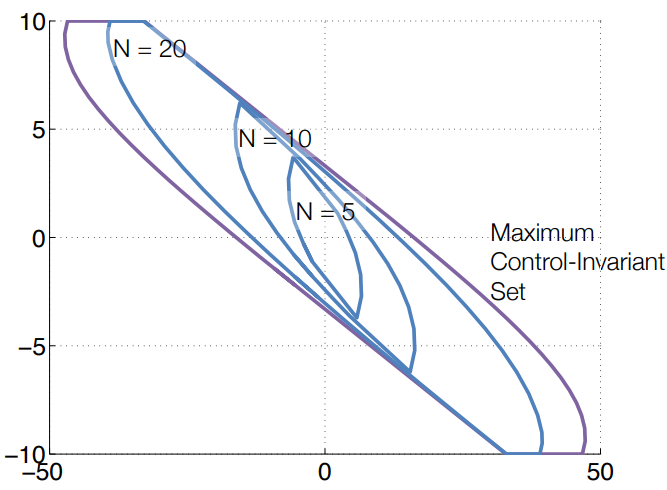
\includegraphics[width=0.5\textwidth]{images/ch07_zero_terminal_horizon_region.png}
    \caption{Impact of the horizon length with the zero terminal constraint. Increasing \(N\)
    enlarges the feasible region and therefore the certified region of attraction. The figure also
    shows the maximum control-invariant set, which represents the largest set from which
    constraint satisfaction can in principle be maintained indefinitely.}
    \label{fig:ch07_zero_terminal_horizon_region}
\end{figure}

This example motivates the next step. Instead of forcing the terminal state to be exactly equal
to zero, we can require it to lie in a terminal set \(\cX_f\). If this terminal set is invariant under
a suitable local controller, then recursive feasibility and stability can still be proven, while the
region of attraction can be significantly larger.

\subsection{General Terminal Sets}

The zero terminal constraint \(x_N=0\) gives a clean and intuitive stability proof, but it can be
very restrictive. Requiring the predicted state to reach the origin exactly at the end of the
horizon may considerably reduce the feasible set, especially when the horizon is short. The
natural generalization is therefore to replace the terminal equality constraint by a terminal set
constraint
\[
    x_N \in \cX_f .
\]
The goal is to choose \(\cX_f\) so that it enlarges the region of attraction, while still allowing
the same recursive-feasibility and Lyapunov-stability argument to go through.\\

The idea is the following. Instead of asking the MPC optimization to drive the state all the way
to the origin in \(N\) steps, we only ask it to drive the state into a region \(\cX_f\) where a known
local controller can safely take over. This terminal set should be chosen so that, once the state
enters \(\cX_f\), there exists an admissible control law that keeps the state inside \(\cX_f\) and
continues decreasing an appropriate terminal cost. Thus, the terminal set represents a region in
which the infinite-horizon tail of the problem is already under control.\\
For example, in the double integrator case, replacing \(x_N=0\) by \(x_N\in\cX_f\) can enlarge
the feasible set significantly. The optimization problem no longer needs to reach the origin
exactly within the horizon; it only needs to reach a set from which constraint satisfaction and
stability can be guaranteed afterwards. This is precisely why terminal sets are useful in MPC:
they make the finite-horizon problem less conservative while preserving the theoretical
guarantees.

\subsubsection{Invariant terminal sets}

The required property of the terminal set is positive invariance under a local terminal control
law. Recall that a set \(\mathcal{O}\) is positively invariant for a closed-loop system
\[
    x(k+1)=g_{\mathrm{cl}}(x(k))
\]
if
\[
    x(0)\in\mathcal{O}
    \quad\Longrightarrow\quad
    x(k)\in\mathcal{O}
    \qquad \forall k\in\mathbb{N}_+.
\]
The largest closed positively invariant set, when it exists, is called the maximal positively
invariant set and is denoted by \(\mathcal{O}_\infty\).\\
In the MPC terminal-set construction, the closed-loop system inside the terminal set is generated
by a local feedback law
\[
    \kappa_f(x).
\]
Thus, for the linear system
\[
    x^+ = Ax+B u,
\]
we require
\[
    Ax+B\kappa_f(x)\in\cX_f,
    \qquad \forall x\in\cX_f.
\]
In addition, the terminal controller must satisfy the original constraints in the terminal set:
\[
    \cX_f\subseteq \cX,
    \qquad
    \kappa_f(x)\in\cU,
    \qquad \forall x\in\cX_f.
\]
These conditions mean that, once the predicted state reaches \(\cX_f\), the terminal controller
can keep the state feasible forever. This is the key replacement for the simple condition
\(x_N=0\) used in the previous proof.

\begin{theorembox}[Invariant terminal set]
A terminal set \(\cX_f\) is suitable for the MPC stability proof if there exists a local controller
\(\kappa_f\) such that
\[
    Ax+B\kappa_f(x)\in\cX_f,
    \qquad \forall x\in\cX_f,
\]
and
\[
    \cX_f\subseteq\cX,
    \qquad
    \kappa_f(x)\in\cU,
    \qquad \forall x\in\cX_f.
\]
Thus, inside \(\cX_f\), the local controller preserves both invariance and constraint satisfaction.
\end{theorembox}

\subsubsection{Main stability result}

We now state the standard sufficient conditions for recursive feasibility and asymptotic stability
of MPC with a general terminal set. Consider the finite-horizon problem
\[
\begin{aligned}
    J^\star(x(k))
    =
    \min_U \quad
    & \terminalcost(x_N)
    +
    \sum_{i=0}^{N-1}\stagecost(x_i,u_i)\\
    \text{subj. to}\quad
    & x_{i+1}=Ax_i+Bu_i,
    \qquad i=0,\ldots,N-1,\\
    & x_i\in\cX,\qquad u_i\in\cU,
    \qquad i=0,\ldots,N-1,\\
    & x_N\in\cX_f,\\
    & x_0=x(k).
\end{aligned}
\]
The first assumption is that the stage cost is positive definite, meaning that it is zero at the
origin and strictly positive away from it. In the regulation setting this can be expressed as
\[
    \stagecost(0,0)=0,
    \qquad
    \stagecost(x,u)>0
    \quad\text{for } (x,u)\neq(0,0).
\]
The second assumption is the invariance and constraint-satisfaction property of the terminal
set:
\[
    Ax+B\kappa_f(x)\in\cX_f,
    \qquad \forall x\in\cX_f,
\]
with
\[
    \cX_f\subseteq\cX,
    \qquad
    \kappa_f(x)\in\cU,
    \qquad \forall x\in\cX_f.
\]
The third assumption concerns the terminal cost. The terminal cost must be a Lyapunov
function for the terminal closed loop inside \(\cX_f\). More precisely, it must satisfy
\[
    \terminalcost(Ax+B\kappa_f(x))-\terminalcost(x)
    \leq
    -\stagecost(x,\kappa_f(x)),
    \qquad \forall x\in\cX_f.
\]
This inequality says that the decrease of the terminal cost along the local terminal controller
is large enough to pay for the stage cost incurred at the terminal state. Therefore, the terminal
cost behaves as an upper approximation of the infinite-horizon cost-to-go after the end of the
prediction horizon.

\begin{theorembox}[MPC feasibility and stability theorem]
Assume that the stage cost is positive definite. Assume also that there exists a local terminal
control law \(\kappa_f\) such that the terminal set \(\cX_f\) is invariant under
\[
    x^+ = Ax+B\kappa_f(x),
\]
and such that all state and input constraints are satisfied in \(\cX_f\). Finally, assume that the
terminal cost satisfies
\[
    \terminalcost(Ax+B\kappa_f(x))-\terminalcost(x)
    \leq
    -\stagecost(x,\kappa_f(x)),
    \qquad \forall x\in\cX_f.
\]
Then the closed-loop system under the MPC law
\[
    u(k)=u_0^\star(x(k))
\]
is asymptotically stable on the feasible set \(X_N\). Moreover, \(X_N\) is positive invariant for
the closed-loop system
\[
    x(k+1)=Ax(k)+Bu_0^\star(x(k)).
\]
\end{theorembox}

\subsubsection{Proof idea}

The proof follows the same structure as in the zero terminal constraint case. The only difference
is that the last element of the shifted sequence is no longer the zero input. Instead, it is the
terminal control law evaluated at the old terminal state.

Assume that the MPC problem is feasible at \(x(k)\), and let
\[
    \{u_0^\star,u_1^\star,\ldots,u_{N-1}^\star\}
\]
be the optimal input sequence computed at \(x(k)\). Let the associated predicted state trajectory
be
\[
    \{x(k),x_1^\star,\ldots,x_N^\star\}.
\]
Since the terminal constraint is satisfied, we have
\[
    x_N^\star\in\cX_f.
\]
The MPC controller applies
\[
    u(k)=u_0^\star,
\]
so that the true successor state is
\[
    x(k+1)=Ax(k)+Bu_0^\star=x_1^\star.
\]

At time \(k+1\), we construct a candidate input sequence by shifting the old optimal sequence
and appending the terminal controller:
\[
    \widetilde{U}
    =
    \{u_1^\star,u_2^\star,\ldots,u_{N-1}^\star,\kappa_f(x_N^\star)\}.
\]
The first \(N-1\) inputs reproduce the tail of the old feasible trajectory. The last input is
feasible because \(x_N^\star\in\cX_f\) and, by construction,
\[
    \kappa_f(x_N^\star)\in\cU.
\]
Moreover, the successor of the old terminal state satisfies
\[
    Ax_N^\star+B\kappa_f(x_N^\star)\in\cX_f,
\]
because \(\cX_f\) is invariant under the terminal controller. Therefore the shifted sequence
satisfies the terminal constraint at time \(k+1\). This proves recursive feasibility.

The stability part uses the same candidate sequence. At time \(k\), the optimal cost is
\[
    J^\star(x(k))
    =
    \sum_{i=0}^{N-1}\stagecost(x_i^\star,u_i^\star)
    +
    \terminalcost(x_N^\star).
\]
At the next state \(x(k+1)=x_1^\star\), the shifted sequence is feasible, but not necessarily
optimal. Hence the optimal cost at \(x(k+1)\) is bounded above by the cost of this candidate:
\[
\begin{aligned}
    J^\star(x(k+1))
    \leq\;&
    \sum_{i=1}^{N-1}\stagecost(x_i^\star,u_i^\star)
    +
    \stagecost(x_N^\star,\kappa_f(x_N^\star))\\
    &+
    \terminalcost(Ax_N^\star+B\kappa_f(x_N^\star)).
\end{aligned}
\]
We rewrite this expression by adding and subtracting the old cost:
\[
\begin{aligned}
    J^\star(x(k+1))
    \leq\;&
    J^\star(x(k))
    -
    \stagecost(x_0^\star,u_0^\star)\\
    &+
    \terminalcost(Ax_N^\star+B\kappa_f(x_N^\star))
    -
    \terminalcost(x_N^\star)\\
    &+
    \stagecost(x_N^\star,\kappa_f(x_N^\star)).
\end{aligned}
\]
The last two terms are nonpositive by the terminal Lyapunov condition:
\[
    \terminalcost(Ax_N^\star+B\kappa_f(x_N^\star))
    -
    \terminalcost(x_N^\star)
    +
    \stagecost(x_N^\star,\kappa_f(x_N^\star))
    \leq 0.
\]
Therefore
\[
    J^\star(x(k+1))-J^\star(x(k))
    \leq
    -\stagecost(x(k),u_0^\star).
\]
Since the stage cost is positive definite, this is a strict decrease away from the origin. Thus
the optimal value function \(J^\star\) is a Lyapunov function for the MPC closed loop, and the
closed-loop system is asymptotically stable on \(X_N\).

\begin{theorembox}[Shifted-sequence proof]
The proof is based on the candidate sequence
\[
    \widetilde{U}
    =
    \{u_1^\star,\ldots,u_{N-1}^\star,\kappa_f(x_N^\star)\}.
\]
The terminal constraint gives recursive feasibility because \(x_N^\star\in\cX_f\) implies
\[
    Ax_N^\star+B\kappa_f(x_N^\star)\in\cX_f.
\]
The terminal-cost decrease condition gives Lyapunov decrease because it cancels the additional
terminal stage cost. Hence \(J^\star\) becomes a Lyapunov function for the MPC closed loop.
\end{theorembox}

\subsubsection{Choice of Terminal Set and Cost for Linear Systems with Quadratic Cost}

We now specialize the previous result to the most common linear-quadratic MPC setting. The
finite-horizon problem is
\[
\begin{aligned}
    J^\star(x(k))
    =
    \min_U \quad
    & x_N^\top P x_N
    +
    \sum_{i=0}^{N-1}
    \left(
        x_i^\top Qx_i+u_i^\top Ru_i
    \right)\\
    \text{subj. to}\quad
    & x_{i+1}=Ax_i+Bu_i,
    \qquad i=0,\ldots,N-1,\\
    & x_i\in\cX,\qquad u_i\in\cU,
    \qquad i=0,\ldots,N-1,\\
    & x_N\in\cX_f,\\
    & x_0=x(k).
\end{aligned}
\]
Here
\[
    Q=Q^\top\succeq 0,
    \qquad
    R=R^\top\succ 0.
\]
A standard design is obtained by using the unconstrained infinite-horizon LQR controller as the
terminal controller. Let \(P_\infty\) solve the discrete-time algebraic Riccati equation
\[
    P_\infty
    =
    A^\top P_\infty A
    +
    Q
    -
    A^\top P_\infty B
    (B^\top P_\infty B+R)^{-1}
    B^\top P_\infty A.
\]
The corresponding LQR feedback gain is
\[
    F_\infty
    =
    -(B^\top P_\infty B+R)^{-1}B^\top P_\infty A.
\]
We then choose the terminal cost and terminal controller as
\[
    P=P_\infty,
    \qquad
    \terminalcost(x)=x^\top P_\infty x,
    \qquad
    \kappa_f(x)=F_\infty x.
\]

The terminal set \(\cX_f\) is chosen as an invariant set for the LQR closed-loop system
\[
    x^+=(A+BF_\infty)x.
\]
In addition, the state and input constraints must be satisfied in \(\cX_f\). If
\[
    \cX=\{x\mid A_xx\leq b_x\},
    \qquad
    \cU=\{u\mid A_uu\leq b_u\},
\]
then the admissible closed-loop constraint set for the terminal controller is
\[
    \cX_{\mathrm{cl}}
    :=
    \left\{
        x
        \,\middle|\,
        \begin{bmatrix}
            A_x\\
            A_uF_\infty
        \end{bmatrix}x
        \leq
        \begin{bmatrix}
            b_x\\
            b_u
        \end{bmatrix}
    \right\}.
\]
A natural choice is to take \(\cX_f\) as the maximal invariant set for
\[
    x^+=(A+BF_\infty)x
\]
inside \(\cX_{\mathrm{cl}}\). By construction, this gives
\[
    (A+BF_\infty)x\in\cX_f,
    \qquad \forall x\in\cX_f,
\]
and
\[
    \cX_f\subseteq\cX,
    \qquad
    F_\infty x\in\cU,
    \qquad \forall x\in\cX_f.
\]

It remains to verify the terminal-cost condition. Since
\[
    x^+=(A+BF_\infty)x,
\]
we compute
\[
\begin{aligned}
    &(x^+)^\top P_\infty x^+ - x^\top P_\infty x\\
    &\quad =
    x^\top
    \left(
        (A+BF_\infty)^\top P_\infty (A+BF_\infty)
        -
        P_\infty
    \right)x.
\end{aligned}
\]
Using the Riccati equation and the definition of \(F_\infty\), this becomes
\[
    (x^+)^\top P_\infty x^+ - x^\top P_\infty x
    =
    -x^\top\left(Q+F_\infty^\top R F_\infty\right)x.
\]
Since
\[
    \stagecost(x,F_\infty x)
    =
    x^\top Qx + x^\top F_\infty^\top R F_\infty x,
\]
we obtain
\[
    \terminalcost((A+BF_\infty)x)-\terminalcost(x)
    =
    -\stagecost(x,F_\infty x).
\]
Thus the terminal cost is a Lyapunov function for the terminal controller in \(\cX_f\), and the
terminal-cost decrease assumption is satisfied exactly.

\begin{theorembox}[Linear-quadratic terminal ingredients]
For linear MPC with quadratic cost, a standard stabilizing choice is
\[
    \kappa_f(x)=F_\infty x,
    \qquad
    \terminalcost(x)=x^\top P_\infty x,
\]
where \(F_\infty\) and \(P_\infty\) are obtained from the unconstrained infinite-horizon LQR
problem. The terminal set \(\cX_f\) is chosen as an invariant set for
\[
    x^+=(A+BF_\infty)x
\]
inside the set where both \(x\in\cX\) and \(F_\infty x\in\cU\). With these choices, all assumptions
of the MPC feasibility and stability theorem are verified.
\end{theorembox}

\section{Region of Attraction and Practical Remarks}

The feasible set of the MPC problem,
\[
    X_N
    =
    \left\{
        x_0
        \,\middle|\,
        \exists\, u_0,\ldots,u_{N-1}
        \text{ satisfying the dynamics, constraints, and } x_N\in\cX_f
    \right\},
\]
is also the certified region of attraction in the stability theorem. If \(x(0)\in X_N\), then
recursive feasibility ensures that the closed-loop trajectory remains in \(X_N\), and the
Lyapunov decrease of the optimal cost ensures convergence to the origin.\\

The choice of terminal set affects this region significantly. The terminal constraint \(x_N=0\)
is the simplest possible choice, but it can lead to a small feasible set, especially when \(N\) is
short. A larger invariant terminal set generally increases the feasible set, because the predicted
trajectory only needs to reach a region where the local controller can take over, rather than
reach the origin exactly.\\
There is, however, an important practical trade-off. Adding a terminal constraint gives a clean
sufficient condition for feasibility and stability, but it may be conservative. It is possible that
an MPC controller without a terminal constraint has a larger region of attraction in practice,
but characterizing that region is generally difficult. The terminal-set approach sacrifices some
flexibility in exchange for a tractable certificate.\\

For linear systems with quadratic cost, the construction based on LQR and invariant sets gives
a systematic design method. In practice, one often enlarges the horizon and checks closed-loop
behavior by simulation or sampling. As the horizon increases, the region of attraction of the
finite-horizon MPC controller typically approaches the maximal control invariant set associated
with the constraints. However, longer horizons increase computational cost, so the horizon must
be chosen as a compromise between performance, feasibility, stability margin, and online
optimization time.

\section{Extension to Nonlinear MPC}

The stability argument presented above is not fundamentally tied to linear dynamics. Consider
a nonlinear discrete-time system
\[
    x(k+1)=g(x(k),u(k)).
\]
The nonlinear MPC problem can be written as
\[
\begin{aligned}
    J^\star(x(k))
    =
    \min_U \quad
    & \terminalcost(x_N)
    +
    \sum_{i=0}^{N-1}\stagecost(x_i,u_i) \\
    \text{subj. to} \quad
    & x_{i+1}=g(x_i,u_i), \qquad i=0,\ldots,N-1,\\
    & x_i\in\cX,\qquad u_i\in\cU,\qquad i=0,\ldots,N-1,\\
    & x_N\in\cX_f,\\
    & x_0=x(k).
\end{aligned}
\]
The same proof idea applies if there exists a terminal controller \(\kappa_f\) such that
\[
    g(x,\kappa_f(x))\in\cX_f
    \qquad
    \forall x\in\cX_f,
\]
with
\[
    \cX_f\subseteq\cX,
    \qquad
    \kappa_f(x)\in\cU
    \qquad
    \forall x\in\cX_f,
\]
and if the terminal cost satisfies
\[
    \terminalcost(g(x,\kappa_f(x)))-\terminalcost(x)
    \leq
    -\stagecost(x,\kappa_f(x))
    \qquad
    \forall x\in\cX_f.
\]
Then the shifted-sequence argument again proves recursive feasibility, and the optimal value
function again decreases along the closed-loop trajectory.\\
The conceptual extension is therefore direct: Lyapunov stability is a general framework for
nonlinear systems, and the terminal-set/terminal-cost argument only relies on invariance and
cost decrease. The practical difficulty is computational. For nonlinear systems, finding a suitable
terminal set \(\cX_f\), terminal controller \(\kappa_f\), and terminal cost \(\terminalcost\) can be
very challenging. In many applications, one uses local linearization, local LQR design, or other
Lyapunov-based constructions to obtain approximate terminal ingredients near the desired
equilibrium.

\section{Summary}

Finite-horizon MPC is not automatically recursively feasible and not automatically stable. The
reason is that finite-horizon optimization is short-sighted: it optimizes an open-loop prediction
over a finite window, whereas the actual controller is implemented in closed loop by repeatedly
resolving the problem. As a result, the controller may drive the system to a state from which
the next optimization problem is infeasible, or it may generate feasible trajectories that do not
converge to the origin.\\

The infinite-horizon constrained optimal control problem avoids this difficulty conceptually,
because the optimized trajectory already accounts for the entire future. If the infinite-horizon
problem is feasible and has finite cost, the remaining tail of the optimal trajectory provides a
natural feasible continuation after the first input is applied. However, infinite-horizon constrained
problems are generally not computable online.\\
The stabilizing MPC construction mimics the infinite-horizon tail by introducing terminal
ingredients. The terminal set \(\cX_f\) is chosen so that, once the predicted trajectory reaches it,
a known local controller \(\kappa_f\) can keep the system feasible forever. The terminal cost
\(\terminalcost\) is chosen so that it decreases under this terminal controller by at least the
incurred stage cost. These two properties allow one to prove recursive feasibility by shifting the
previous optimal sequence and appending the terminal control input. They also allow one to
prove stability by showing that the optimal MPC value function is a Lyapunov function.\\
For linear systems with quadratic costs, a standard choice is obtained from the unconstrained
infinite-horizon LQR problem. The terminal controller is the LQR feedback \(F_\infty x\), the
terminal cost is \(x^\top P_\infty x\), and the terminal set is an invariant set for the closed-loop
system \(x^+=(A+BF_\infty)x\) satisfying the state and input constraints. This construction
verifies the assumptions of the general MPC stability theorem and provides a systematic way to
design stabilizing finite-horizon MPC.\\

The same ideas extend to nonlinear MPC, because the proof relies on invariance and Lyapunov
decrease rather than on linearity. The main challenge in the nonlinear case is the computation
of suitable terminal sets, terminal controllers, and terminal costs.